% Sketch output, version 0.3 (build 2d, Wed Apr 20 23:38:45 2011)
% Output language: PGF/TikZ,LaTeX
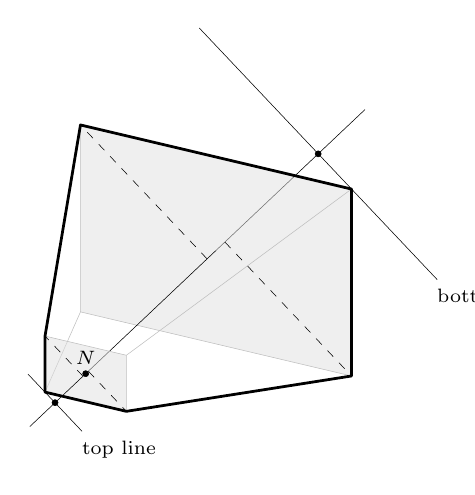
\begin{tikzpicture}[line join=round,line width=0.2pt,>=latex]
\draw(2.364,2.236)--(4.256,4.025);
\filldraw[color=lightgray,fill=lightgray!50,fill opacity=0.5](4.085,3.016)--(.643,3.83)--(.643,1.456)--(4.085,.642)--cycle;
\draw[color=lightgray](.193,.437)--(.643,1.456);
\draw[color=lightgray](.193,1.149)--(.643,3.83);
\draw(.709,.671)--(2.364,2.236);
\draw[color=lightgray](1.226,.193)--(4.085,.642);
\draw[color=lightgray](1.226,.905)--(4.085,3.016);
\filldraw[color=lightgray,fill=lightgray!50,fill opacity=0.5](1.226,.905)--(.193,1.149)--(.193,.437)--(1.226,.193)--cycle;
\draw(0,0)--(.709,.671);
\draw[solid](2.151,5.062)--(5.174,1.865);
\filldraw(3.662,3.463) circle (1.1pt);
\draw[dashed](2.477,2.343)--(4.085,.642);
\draw[dashed](2.251,2.129)--(.643,3.83);
\draw[dashed](.743,.703)--(1.226,.193);
\draw[dashed](.675,.639)--(.193,1.149);
\draw[solid](-.024,.666)--(.663,-.061);
\filldraw(.32,.303) circle (1.1pt);
\filldraw[](.709,.671) circle (1.1pt);
\filldraw[fill=none,line width=1pt](.643,3.83)--(.193,1.149)--(.193,.437)--(1.226,.193)--(4.085,.642)--(4.085,3.016)--cycle;

    \coordinate [label=90:\scriptsize$N$] (N) at (.709,.671);
    \coordinate [label=-90:{\makebox[0pt][l]{\scriptsize top line}}] (top) at (.663,-.061);
    \coordinate [label=-90:{\makebox[0pt][l]{\scriptsize bottom line}}] (bot) at (5.174,1.865);
  \end{tikzpicture}% End sketch output
